\subsection{Potencial Hidrogenônico (pH)}

A escala de pH (Potencial Hidrogenônico) é um conceito bastante estudado em química. Esse conceito foi definido pelo químico dinamarquês Soren Peter Lauritz Sorensen no ano de 1909. Ela serve para determinar os níveis de acidez de uma solução. O pH de uma solução é definido como o logaritmo decimal do inverso da concentração de $H_3O^{+}$ (ion hidroxônio), ou seja,

\[
pH = - \log[H_3O^{+}]
\]

Assim, percebe-se que quanto maior o valor da concentração de $H_3O^{+}$, menor o valor do pH, ou seja, quanto mais ácida a solução, menor o pH. Definir a acidez em uma escala logarítimica foi muito positivo. Primeiro que, em solução, os valores de íons hidrogênio podem variar drasticamente, além de serem, na maioria das vezes, expressos em potências negativas de 10.


A classificação do pH se dá da seguinte forma:

\begin{center}
\begin{tabular}{|c|c|}
\hline
\textbf{pH} & \textbf{solução} \\
\hline
0 a 7 & ácida \\
\hline
7 & neutra \\
\hline
7 a 14 & básica \\
\hline
\end{tabular}
\end{center}

% \begin{figure}[H]
%     \centering
%     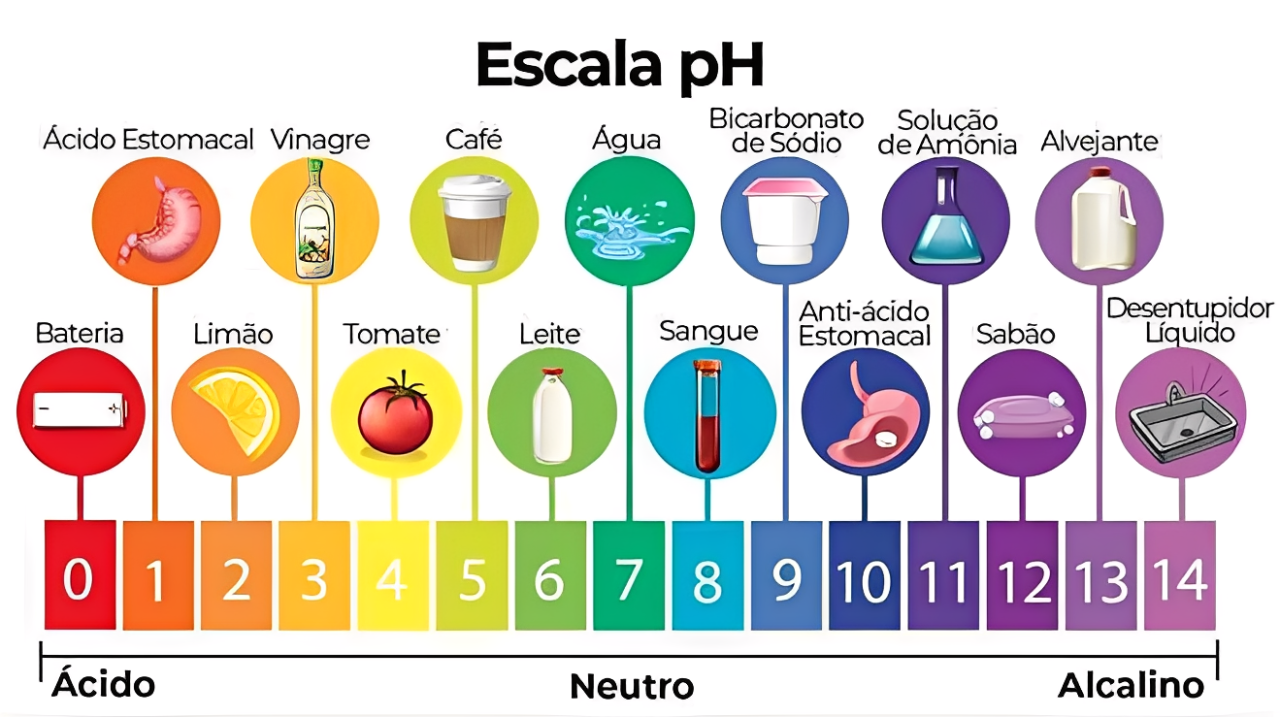
\includegraphics[width=\linewidth]{img/escalaph.jpg}
%     \caption{Escala pH}
% \end{figure}
Abaixo temos uma imagem com o pH de algumas soluções mais comuns.

\begin{figure}[h]
    \centering
    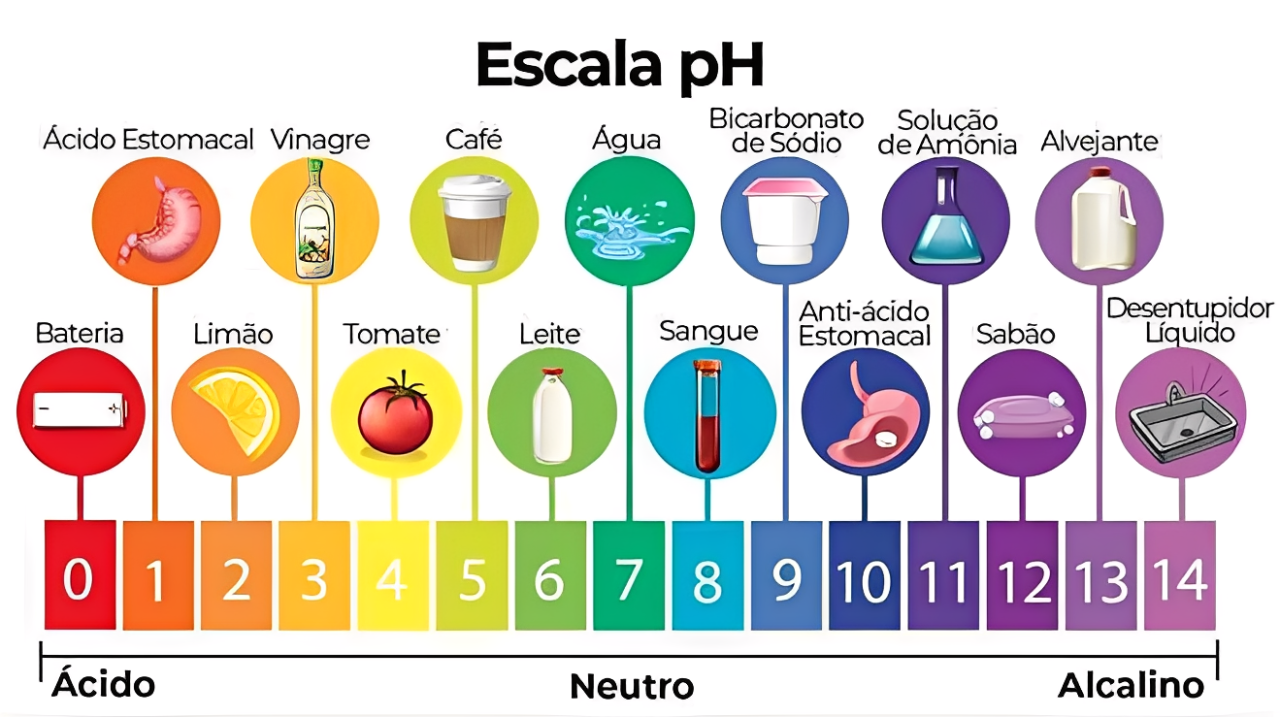
\includegraphics[width=0.9\textwidth]{img/escalaph.png}
    \caption{Exemplos de soluções e seu pH}
    \label{fig:escalaph}
\end{figure}


\textbf{Exemplo.} Jean, um químico curioso, estava na praia e enche um copo com água do mar. Ao chegar em seu laboratório, ele mede a concentração de íons ($H_3O^{+}$) desse copo de água, obteve-se que esta é de $10^{-8}$ mol/l. Assim qual será o pH dessa água? 

\begin{align*}
pH &= -\log[H_3O^+], \\
pH &= -\log 10^{-8}, \\
pH &= -(-8) \log 10, \\
pH &= 8
\end{align*}

Assim, Jean notou que a água do mar era uma solução básica.


